\section{Linked Lists}

\begin{frame}{Linked Lists}{Introduction}
  \textbf{Linked list:}
  \begin{itemize}
    \item<2->
      Dynamic datastructure
    \item<3->
      Number of elements changeable
    \item<4->
      Data elements can be simple types or composed datastructures
    \item<5->
      Elements are linked through references / pointer to the predecessor /
      successor
    \item<6->
      Single / Doubly linked lists possible
  \end{itemize}
  \onslide<7->
  \begin{figure}
    \begin{adjustbox}{width=\linewidth}%
\begin{tikzpicture}[
  element/.style={
    draw={Mittel-Blau},
    fill={white},
    line width=0.075em
  }, element_link/.style={
    draw={Mittel-Blau},
    fill={Hell-Blau},
    line width=0.075em
  }, arrow/.style={
    draw={Mittel-Blau},
    line width=0.125em
  }
]%
\foreach \x in {4,3,...,-1}{
  \ifnum \x>-1
    \ifnum \x=3 \else
      \draw[element_link] (1.5*\x, 1.0) rectangle (1.5*\x + 1.0, 0.75);
      \draw[element] (1.5*\x, 0.25) rectangle (1.5*\x + 1.0, 0.75);
    \fi
  \fi
  
  \draw[->, arrow] (1.5*\x + 1.0, 0.875) -- (1.5*\x + 1.5, 0.875);
}

\draw (5.0, 0.5) node {\footnotesize ...};
\draw (-0.5, 0.875) node[anchor=east] {\footnotesize \texttt{first}};
\draw (7.5, 0.875)
  node[anchor=west] {\footnotesize\texttt{\color{Mittel-Blau}None}};

\draw (3.5, 1.0) node[anchor=south] {\footnotesize Pointer to next element};
\draw (3.5, 0.5) node {\footnotesize Data};
\end{tikzpicture}%
\end{adjustbox}%
    \caption{Linked list}
    \label{fig:linked_list:singly_linked_list}
  \end{figure}
\end{frame}

%-------------------------------------------------------------------------------

\begin{frame}{Linked Lists}{Introduction}
  \textbf{Properties in comperison to an array:}
  \begin{itemize}
    \item<2->
      Minimal extra space for storing pointer
    \item<3->
      We do not need to copy elements on {\color{Mittel-Blau}\texttt{insert}}
      or {\color{Mittel-Blau}\texttt{remove}}
    \item<4->
      The number of elements can be simply modified 
    \item<5->
      No direct access of elements\\
      $\Rightarrow$ We have to iterate over the list
  \end{itemize}
\end{frame}

%-------------------------------------------------------------------------------

\begin{frame}{Linked Lists}{Variation}
  \textbf{List with head / last element pointer:}
   \onslide<2->
  \begin{figure}
    \begin{adjustbox}{width=\linewidth}%
\begin{tikzpicture}[
  element/.style={
    draw={Mittel-Blau},
    fill={white},
    line width=0.075em
  }, element_head/.style={
    draw={Mittel-Blau},
    fill={white},
    pattern=north east lines,
    pattern color={Mittel-Blau},
    line width=0.075em
  }, element_link/.style={
    draw={Mittel-Blau},
    fill={Hell-Blau},
    line width=0.075em
  }, arrow/.style={
    draw={Mittel-Blau},
    line width=0.125em
  }
]%
\foreach \x in {3,2,...,-1}{
  \ifnum \x=2 \else
    \draw[element_link] (1.5*\x, 1.0) rectangle (1.5*\x + 1.0, 0.75);
    \ifnum \x=-1
      \draw[element_head] (1.5*\x, 0.25) rectangle (1.5*\x + 1.0, 0.75);
    \else
      \draw[element] (1.5*\x, 0.25) rectangle (1.5*\x + 1.0, 0.75);
      \ifnum \x<3
        \draw (1.5*\x + 0.5, 0.5) node {\footnotesize \x};
      \else
        \draw (1.5*\x + 0.5, 0.5) node {\footnotesize n};
      \fi
    \fi
  \fi
  
  \draw[->, arrow] (1.5*\x + 1.0, 0.875) -- (1.5*\x + 1.5, 0.875);
}

\draw (3.5, 0.5) node {\footnotesize ...};
\draw (6.5, 0.875) node {\footnotesize\texttt{\color{Mittel-Blau}None}};

\draw (-1.25, 1.25) node[anchor=south] {\footnotesize \texttt{head}};
\draw[->, arrow] (-1.25, 1.25) -- (-1.25, 1.0);
\draw (4.75, 1.25) node[anchor=south] {\footnotesize \texttt{last}};
\draw[->, arrow] (4.75, 1.25) -- (4.75, 1.0);
\end{tikzpicture}%
\end{adjustbox}%
    \caption{Singly linked list}
    \label{fig:linked_list:variation:singly_linked_list_with_head}
  \end{figure}
  \begin{itemize}
    \item<3->
      Head element has pointer to first list element
    \item<4->
      May also hold additional information:
      \begin{itemize}
        \item<5->
          Number of elements
      \end{itemize}
  \end{itemize}
\end{frame}

%-------------------------------------------------------------------------------

\begin{frame}{Linked Lists}{Variation}
  \textbf{Doubly linked list:}
  \onslide<2->
    \begin{figure}
    \begin{adjustbox}{width=\linewidth}%
\begin{tikzpicture}[
  element/.style={
    draw={Mittel-Blau},
    fill={white},
    line width=0.075em
  }, element_head/.style={
    draw={Mittel-Blau},
    fill={white},
    pattern=north east lines,
    pattern color={Mittel-Blau},
    line width=0.075em
  }, element_link/.style={
    draw={Mittel-Blau},
    fill={Hell-Blau},
    line width=0.075em
  }, arrow/.style={
    draw={Mittel-Blau},
    line width=0.125em
  }
]%
% Draw elements
\foreach \x in {4,3,...,0}{
  \ifnum \x=3 \else
    \draw[element_link] (1.5*\x, 0.5) rectangle (1.5*\x + 1.0, 0.75);
    \draw[element_link] (1.5*\x, 1.0) rectangle (1.5*\x + 1.0, 0.75);
    \draw[element] (1.5*\x, 0.0) rectangle (1.5*\x + 1.0, 0.5);
    
    \ifnum \x<4
      \draw (1.5*\x + 0.5, 0.25) node {\footnotesize \x};
    \else
      \draw (1.5*\x + 0.5, 0.25) node {\footnotesize $n$};
    \fi
    
    \draw[->, arrow] (1.5*\x + 0.5, 1.5) -- (1.5*\x + 0.5, 1.0);
  \fi
  
  \ifnum \x<4
    \draw[->, arrow] (1.5*\x + 1.0, 0.875) -- (1.5*\x + 1.5, 0.875);
    \draw[<-, arrow] (1.5*\x + 1.0, 0.625) -- (1.5*\x + 1.5, 0.625);
  \fi
}

% Pointer
\draw[->, arrow] (7.0, 0.875) -- (7.5, 0.875) -- (7.5, -0.5) --
  (-0.5, -0.5) -- (-0.5, 0.875) -- (0.0, 0.875);
\draw[<-, arrow] (7.0, 0.625) -- (7.25, 0.625) -- (7.25, -0.25) --
  (-0.25, -0.25) -- (-0.25, 0.625) -- (0.0, 0.625);

\draw (5.0, 0.5) node {\footnotesize ...};

% Draw navigation structure
\draw[element] (0.0, 1.5) rectangle (7.0, 2.25);
\draw (3.5, 1.825) node {\footnotesize tree navigation structre};
\end{tikzpicture}%
\end{adjustbox}%4
    \caption{Doubly linked list}
    \label{fig:linked_list:variation:doubly_linked_list}
  \end{figure}
  \begin{itemize}
    \item<3->
      Pointer to successor element
    \item<4->
      Pointer to predecessor element
    \item<5->
      Iterate forward and backward
  \end{itemize}
\end{frame}


%-------------------------------------------------------------------------------

\begin{frame}[fragile]{Linked Lists}{Implementation - Node/Element - Java}
  \small{
  \lstinputlisting[
    language=Java,
    tabsize=4,
    style={java-eclipse-code},
    breaklines=false,
    mathescape=true,
    escapechar={@},
    emph={value, next},
    emphstyle=\color{java_static}
  ]{Code/LinkedList/NodePart1new.java}}
\end{frame}

%-------------------------------------------------------------------------------

\begin{frame}[fragile]{Linked Lists}{Implementation - Node/Element - Java}
  \vspace{-1.125em}
  \lstinputlisting[
    language=Java,
    tabsize=4,
    style={java-eclipse-code},
    breaklines=false,
    mathescape=true,
    escapechar={@},
    emph={value, next},
    emphstyle=\color{java_static}
  ]{Code/LinkedList/NodePart2new.java}
\end{frame}

%-------------------------------------------------------------------------------

%% \begin{frame}[fragile]{Linked Lists}{Implementation - Node - Java}
%%   \lstinputlisting[
%%     language=Java,
%%     tabsize=4,
%%     style={java-eclipse-code},
%%     breaklines=false,
%%     mathescape=true,
%%     escapechar={@},
%%     emph={value, next},
%%     emphstyle=\color{java_static}
%%   ]{Code/LinkedList/NodePart3.java}
%% \end{frame}

%-------------------------------------------------------------------------------

%% \begin{frame}[fragile]{Linked Lists}{Implementation - Node/Element - C++ - Header}
%%   \vspace{-1.125em}
%%   \lstinputlisting[
%%     language=C++,
%%     tabsize=4,
%%     style={cpp-eclipse-code},
%%     breaklines=false,
%%     escapechar={@}
%%   ]{Code/LinkedList/Node.h}
%% \end{frame}

%-------------------------------------------------------------------------------

\begin{frame}[fragile]{Linked Lists}{Implementation - Node/Element - C++}
  \lstinputlisting[
    language=C++,
    tabsize=4,
    style={cpp-eclipse-code},
    breaklines=false,
    escapechar={@}
  ]{Code/LinkedList/NodePart1new.cpp}
\end{frame}

%-------------------------------------------------------------------------------

\begin{frame}[fragile]{Linked Lists}{Implementation - Node/Element - C++}
  \lstinputlisting[
    language=C++,
    tabsize=4,
    style={cpp-eclipse-code},
    breaklines=false,
    escapechar={@}
  ]{Code/LinkedList/NodePart2new.cpp}
\end{frame}

%-------------------------------------------------------------------------------

\begin{frame}[fragile]{Linked Lists}{Implementation - Node/Element - Python}
  \lstinputlisting[
    language=Python,
    tabsize=4,
    style={python-idle-code},
    escapechar={@},
    morekeywords={None},
    emph={Node, __init__},
    emphstyle=\color{blue}
  ]{Code/LinkedList/Node.py}
\end{frame}

%-------------------------------------------------------------------------------

\begin{frame}{Linked Lists}{Usage examples}
  \textbf{Creating linked lists  - Python:}
  \begin{itemize}
    \item<2->
      \lstinline[
        language=Python,
        style={python-idle-code}
      ]|first = Node(7)|
      \begin{flushleft}
        \begin{adjustbox}{height=0.1\linewidth}%
\begin{tikzpicture}[
  element/.style={
    draw={Mittel-Blau},
    fill={white},
    line width=0.075em
  }, element_link/.style={
    draw={Mittel-Blau},
    fill={Hell-Blau},
    line width=0.075em
  }, arrow/.style={
    draw={Mittel-Blau},
    line width=0.125em
  }
]%
\foreach \x/\value in {-1/0, 0/7}{
  \ifnum \x>-1
    \draw[element_link] (1.5*\x, 1.0) rectangle (1.5*\x + 1.0, 0.75);
    \draw[element] (1.5*\x, 0.25) rectangle (1.5*\x + 1.0, 0.75);
    
    \draw (1.5*\x + 0.5, 0.5) node {\value};
  \fi
  
  \draw[->, arrow] (1.5*\x + 1.0, 0.875) -- (1.5*\x + 1.5, 0.875);
}

\draw (-0.5, 0.875) node[anchor=east] {\footnotesize \texttt{first}};
\draw (1.5, 0.875) node[anchor=west] {\footnotesize{\color{Mittel-Blau}None}};
\end{tikzpicture}%
\end{adjustbox}%
      \end{flushleft}
      \vspace{0.5em}
    \item<3->
      \lstinline[
        language=Python,
        style={python-idle-code}
      ]|first.nextNode = Node(3)|
      \begin{flushleft}
        \begin{adjustbox}{height=0.1\linewidth}%
\begin{tikzpicture}[
  element/.style={
    draw={Mittel-Blau},
    fill={white},
    line width=0.075em
  }, element_link/.style={
    draw={Mittel-Blau},
    fill={Hell-Blau},
    line width=0.075em
  }, arrow/.style={
    draw={Mittel-Blau},
    line width=0.125em
  }
]%
\foreach \x/\value in {-1/0, 0/7, 1/3}{
  \ifnum \x>-1
    \draw[element_link] (1.5*\x, 1.0) rectangle (1.5*\x + 1.0, 0.75);
    \draw[element] (1.5*\x, 0.25) rectangle (1.5*\x + 1.0, 0.75);
    
    \draw (1.5*\x + 0.5, 0.5) node {\value};
  \fi
  
  \draw[->, arrow] (1.5*\x + 1.0, 0.875) -- (1.5*\x + 1.5, 0.875);
}

\draw (-0.5, 0.875) node[anchor=east] {\footnotesize \texttt{first}};
\draw (3.0, 0.875) node[anchor=west] {\footnotesize{\color{Mittel-Blau}None}};
\end{tikzpicture}%
\end{adjustbox}%
      \end{flushleft}
      \vspace{0.5em}
    \item<4->
      \lstinline[
        language=Python,
        style={python-idle-code}
      ]|first.nextNode.value = 4|
      \begin{flushleft}
        \begin{adjustbox}{height=0.1\linewidth}%
\begin{tikzpicture}[
  element/.style={
    draw={Mittel-Blau},
    fill={white},
    line width=0.075em
  }, element_link/.style={
    draw={Mittel-Blau},
    fill={Hell-Blau},
    line width=0.075em
  }, arrow/.style={
    draw={Mittel-Blau},
    line width=0.125em
  }
]%
\foreach \x/\value in {-1/0, 0/7, 1/4}{
  \ifnum \x>-1
    \draw[element_link] (1.5*\x, 1.0) rectangle (1.5*\x + 1.0, 0.75);
    \draw[element] (1.5*\x, 0.25) rectangle (1.5*\x + 1.0, 0.75);
    
    \draw (1.5*\x + 0.5, 0.5) node {\value};
  \fi
  
  \draw[->, arrow] (1.5*\x + 1.0, 0.875) -- (1.5*\x + 1.5, 0.875);
}

\draw (-0.5, 0.875) node[anchor=east] {\footnotesize \texttt{first}};
\draw (3.0, 0.875) node[anchor=west] {\footnotesize{\color{Mittel-Blau}None}};
\end{tikzpicture}%
\end{adjustbox}%
      \end{flushleft}
  \end{itemize}
\end{frame}

%-------------------------------------------------------------------------------

\begin{frame}{Linked Lists}{Implementation - Insert}
  \textbf{Inserting a node after node \texttt{cur}:}
  \begin{flushleft}
    \begin{adjustbox}{width=\linewidth}%
\begin{tikzpicture}[
  element/.style={
    draw={Mittel-Blau},
    fill={white},
    line width=0.075em
  }, element_link/.style={
    draw={Mittel-Blau},
    fill={Hell-Blau},
    line width=0.075em
  }, arrow/.style={
    draw={Mittel-Blau},
    line width=0.125em
  }
]%
\foreach \x/\value in {-1/0, 0/{$n_0$}, 1/{$n_1$}, 2/{$n_2$}, 3/{$n_3$}}{
  \ifnum \x>-1
    \draw[element_link] (1.5*\x, 1.0) rectangle (1.5*\x + 1.0, 0.75);
    \draw[element] (1.5*\x, 0.25) rectangle (1.5*\x + 1.0, 0.75);
    
    \draw (1.5*\x + 0.5, 0.5) node {\value};
  \fi
  
  \draw[->, arrow] (1.5*\x + 1.0, 0.875) -- (1.5*\x + 1.5, 0.875);
}

\draw (-0.5, 0.875) node[anchor=east] {\footnotesize \texttt{first}};
\draw (6.0, 0.875) node[anchor=west] {\footnotesize{\color{Mittel-Blau}None}};

\draw (1.75, 1.25) node[anchor=south] {\footnotesize \texttt{cur}};
\draw[->, arrow] (1.75, 1.25) -- (1.75, 1.0);
\end{tikzpicture}%
\end{adjustbox}%
  \end{flushleft}
\end{frame}

%-------------------------------------------------------------------------------

\begin{frame}{Linked Lists}{Implementation - Insert}
  \textbf{Inserting a node after node \texttt{cur}:}
  \begin{itemize}
    \item<2->
      \lstinline[
      language=Python,
      style={python-idle-code}
      ]|ins = Node(n)|
  \end{itemize}
  \onslide<3->
  \begin{flushleft}
    \begin{adjustbox}{width=\linewidth}%
\begin{tikzpicture}[
  element/.style={
    draw={Mittel-Blau},
    fill={white},
    line width=0.075em
  }, element_link/.style={
    draw={Mittel-Blau},
    fill={Hell-Blau},
    line width=0.075em
  }, arrow/.style={
    draw={Mittel-Blau},
    line width=0.125em
  }
]%
\foreach \x/\value in {-1/0, 0/{$n_0$}, 1/{$n_1$}, 2/{$n_2$}, 3/{$n_3$}}{
  \ifnum \x>-1
    \draw[element_link] (1.5*\x, 1.0) rectangle (1.5*\x + 1.0, 0.75);
    \draw[element] (1.5*\x, 0.25) rectangle (1.5*\x + 1.0, 0.75);
    
    \draw (1.5*\x + 0.5, 0.5) node {\value};
  \fi
  
  \draw[->, arrow] (1.5*\x + 1.0, 0.875) -- (1.5*\x + 1.5, 0.875);
}
\foreach \x/\value in {-1/0, 0/{$n$}}{
  \ifnum \x>-1
    \draw[element_link]
      (1.5*\x, 1.0 + 1.5) rectangle (1.5*\x + 1.0, 0.75 + 1.5);
    \draw[element] (1.5*\x, 0.25 + 1.5) rectangle (1.5*\x + 1.0, 0.75 + 1.5);
    
    \draw (1.5*\x + 0.5, 0.5 + 1.5) node {\value};
  \fi
  
  \draw[->, arrow] (1.5*\x + 1.0, 0.875 + 1.5) -- (1.5*\x + 1.5, 0.875 + 1.5);
}

\draw (-0.5, 0.875) node[anchor=east] {\footnotesize \texttt{first}};
\draw (6.0, 0.875) node[anchor=west] {\footnotesize{\color{Mittel-Blau}None}};

\draw (-0.5, 0.875 + 1.5) node[anchor=east] {\footnotesize \texttt{ins}};
\draw (1.5, 0.875 + 1.5)
  node[anchor=west] {\footnotesize{\color{Mittel-Blau}None}};

\draw (1.75, 1.25) node[anchor=south] {\footnotesize \texttt{cur}};
\draw[->, arrow] (1.75, 1.25) -- (1.75, 1.0);
\end{tikzpicture}%
\end{adjustbox}%
  \end{flushleft}
\end{frame}

%-------------------------------------------------------------------------------

\begin{frame}{Linked Lists}{Implementation - Insert}
  \textbf{Inserting a node after node \texttt{cur}:}
  \begin{itemize}
    \item<2->
      \lstinline[
        language=Python,
        style={python-idle-code}
      ]|ins.nextNode = cur.nextNode|
  \end{itemize}
  \onslide<3->
  \begin{flushleft}
    \begin{adjustbox}{width=\linewidth}%
\begin{tikzpicture}[
  element/.style={
    draw={Mittel-Blau},
    fill={white},
    line width=0.075em
  }, element_link/.style={
    draw={Mittel-Blau},
    fill={Hell-Blau},
    line width=0.075em
  }, arrow/.style={
    draw={Mittel-Blau},
    line width=0.125em
  }, arrow_new/.style={
    draw={Mittel-Gruen},
    line width=0.125em
  }
]%
\foreach \x/\value in {-1/0, 0/{$n_0$}, 1/{$n_1$}, 2/{$n_2$}, 3/{$n_3$}}{
  \ifnum \x>-1
    \draw[element_link] (1.5*\x, 1.0) rectangle (1.5*\x + 1.0, 0.75);
    \draw[element] (1.5*\x, 0.25) rectangle (1.5*\x + 1.0, 0.75);
    
    \draw (1.5*\x + 0.5, 0.5) node {\value};
  \fi
  
  \draw[->, arrow] (1.5*\x + 1.0, 0.875) -- (1.5*\x + 1.5, 0.875);
}
\foreach \x/\value in {0/{$n$}}{
  \ifnum \x>-1
    \draw[element_link]
      (1.5*\x + 2.25, 1.0 + 1.5) rectangle (1.5*\x + 3.25, 0.75 + 1.5);
    \draw[element]
      (1.5*\x + 2.25, 0.25 + 1.5) rectangle (1.5*\x + 3.25, 0.75 + 1.5);
    
    \draw (1.5*\x + 2.75, 0.5 + 1.5) node {\value};
  \fi
  
  \draw[->, arrow] (1.5*\x + 1.75, 0.875 + 1.5) -- (1.5*\x + 2.25, 0.875 + 1.5);
}

\draw (-0.5, 0.875) node[anchor=east] {\footnotesize \texttt{first}};
\draw (6.0, 0.875) node[anchor=west] {\footnotesize{\color{Mittel-Blau}None}};

\draw (1.75, 0.875 + 1.5) node[anchor=east] {\footnotesize \texttt{ins}};
\draw[->, arrow_new]
  (3.25, 0.875 + 1.5) -- (3.75, 0.875 + 1.5)  -- (3.75, 1.0);

\draw (1.75, 1.25) node[anchor=south] {\footnotesize \texttt{cur}};
\draw[->, arrow] (1.75, 1.25) -- (1.75, 1.0);
\end{tikzpicture}%
\end{adjustbox}%
  \end{flushleft}
\end{frame}

%-------------------------------------------------------------------------------

\begin{frame}{Linked Lists}{Implementation - Insert}
  \textbf{Inserting a node after node \texttt{cur}:}
  \begin{itemize}
    \item<2->
      \lstinline[
        language=Python,
        style={python-idle-code}
      ]|cur.nextNode = ins|
  \end{itemize}
  \onslide<3->
  \begin{flushleft}
    \begin{adjustbox}{width=\linewidth}%
\begin{tikzpicture}[
  element/.style={
    draw={Mittel-Blau},
    fill={white},
    line width=0.075em
  }, element_link/.style={
    draw={Mittel-Blau},
    fill={Hell-Blau},
    line width=0.075em
  }, arrow/.style={
    draw={Mittel-Blau},
    line width=0.125em
  }, arrow_new/.style={
    draw={Mittel-Gruen},
    line width=0.125em
  }
]%
\foreach \x/\value in {-1/0, 0/{$n_0$}, 1/{$n_1$}, 2/{$n_2$}, 3/{$n_3$}}{
  \ifnum \x>-1
    \draw[element_link] (1.5*\x, 1.0) rectangle (1.5*\x + 1.0, 0.75);
    \draw[element] (1.5*\x, 0.25) rectangle (1.5*\x + 1.0, 0.75);
    
    \draw (1.5*\x + 0.5, 0.5) node {\value};
  \fi
  
  \ifnum \x=1 \else
    \draw[->, arrow] (1.5*\x + 1.0, 0.875) -- (1.5*\x + 1.5, 0.875);
  \fi
}
\foreach \x/\value in {0/{$n$}}{
  \draw[element_link]
    (1.5*\x + 2.25, 1.0 + 1.5) rectangle (1.5*\x + 3.25, 0.75 + 1.5);
  \draw[element]
    (1.5*\x + 2.25, 0.25 + 1.5) rectangle (1.5*\x + 3.25, 0.75 + 1.5);
  
  \draw (1.5*\x + 2.75, 0.5 + 1.5) node {\value};
}

\draw (-0.5, 0.875) node[anchor=east] {\footnotesize \texttt{first}};
\draw (6.0, 0.875) node[anchor=west] {\footnotesize{\color{Mittel-Blau}None}};

\draw (1.5, 0.95 + 1.5) node[anchor=east] {\footnotesize \texttt{ins}};
\draw[->, arrow] (1.5, 0.95 + 1.5) -- (2.25, 0.95 + 1.5);
\draw[->, arrow_new]
  (2.5, 0.875) -- (2.75, 0.875) -- (2.75, 1.5)  -- (2.0, 1.5) --
  (2.0, 0.8 + 1.5) -- (2.25, 0.8 + 1.5);

\draw[->, arrow_new] (3.25, 0.875 + 1.5) -- (3.75, 0.875 + 1.5)  -- (3.75, 1.0);

\draw (1.5, 1.5) node[anchor=east] {\footnotesize \texttt{cur}};
\draw[->, arrow] (1.5, 1.5) -- (1.75, 1.5) -- (1.75, 1.0);
\end{tikzpicture}%
\end{adjustbox}%
  \end{flushleft}
\end{frame}

%-------------------------------------------------------------------------------

\begin{frame}{Linked Lists}{Implementation - Insert}
  \textbf{Inserting a node after node \texttt{cur} - single line of code:}
  \onslide<2->
  \begin{figure}
    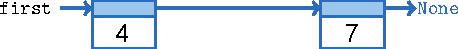
\includegraphics[width=0.5\textwidth]{Images/LinkedList/insert-one-line-pre.pdf}
  \end{figure}
  \begin{itemize}
  \item<3->
    \lstinline[
      language=Python,
      style={python-idle-code}
    ]|cur.nextNode = Node (value ,cur.nextNode )|
  \end{itemize}
  \onslide<4->
  \begin{figure}
    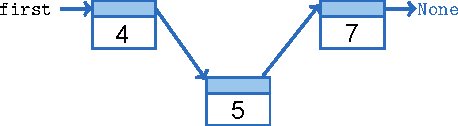
\includegraphics[width=0.5\textwidth]{Images/LinkedList/insert-one-line-post.pdf}
  \end{figure}
\end{frame}

%-------------------------------------------------------------------------------

\begin{frame}{Linked Lists}{Implementation - Remove}
  \textbf{Removing a node \texttt{cur}:}
  \begin{flushleft}
    \begin{adjustbox}{width=\linewidth}%
\begin{tikzpicture}[
  element/.style={
    draw={Mittel-Blau},
    fill={white},
    line width=0.075em
  }, element_link/.style={
    draw={Mittel-Blau},
    fill={Hell-Blau},
    line width=0.075em
  }, arrow/.style={
    draw={Mittel-Blau},
    line width=0.125em
  }
]%
\foreach \x/\value in {-1/0, 0/{$n_0$}, 1/{$n_1$}, 2/{$n_2$}, 3/{$n_3$}}{
  \ifnum \x>-1
    \draw[element_link] (1.5*\x, 1.0) rectangle (1.5*\x + 1.0, 0.75);
    \draw[element] (1.5*\x, 0.25) rectangle (1.5*\x + 1.0, 0.75);
    
    \draw (1.5*\x + 0.5, 0.5) node {\value};
  \fi
  
  \draw[->, arrow] (1.5*\x + 1.0, 0.875) -- (1.5*\x + 1.5, 0.875);
}

\draw (-0.5, 0.875) node[anchor=east] {\footnotesize \texttt{first}};
\draw (6.0, 0.875) node[anchor=west] {\footnotesize{\color{Mittel-Blau}None}};

\draw (1.75 + 1.5, 1.25) node[anchor=south] {\footnotesize \texttt{cur}};
\draw[->, arrow] (1.75 + 1.5, 1.25) -- (1.75 + 1.5, 1.0);
\end{tikzpicture}%
\end{adjustbox}%
  \end{flushleft}
\end{frame}

%-------------------------------------------------------------------------------

\begin{frame}{Linked Lists}{Implementation - Remove}
  \textbf{Removing a node \texttt{cur}:}
  \begin{itemize}
    \item<2->
      Find the predecessor of \texttt{cur}:\\
      \lstinputlisting[
        language=Python,
        tabsize=4,
        style={python-idle-code},
        escapechar={@},
        emphstyle=\color{blue}
      ]{Code/LinkedList/RemoveStep1.py}
    \item<3->
      Runtime of $O(n)$
    \item<4->
      Does not work for first node!
  \end{itemize}
  \vspace{-1.5em}
  \onslide<5->
  \begin{flushleft}
    \begin{adjustbox}{width=\linewidth}%
\begin{tikzpicture}[
  element/.style={
    draw={Mittel-Blau},
    fill={white},
    line width=0.075em
  }, element_link/.style={
    draw={Mittel-Blau},
    fill={Hell-Blau},
    line width=0.075em
  }, arrow/.style={
    draw={Mittel-Blau},
    line width=0.125em
  }
]%
\foreach \x/\value in {-1/0, 0/{$n_0$}, 1/{$n_1$}, 2/{$n_2$}, 3/{$n_3$}}{
  \ifnum \x>-1
    \draw[element_link] (1.5*\x, 1.0) rectangle (1.5*\x + 1.0, 0.75);
    \draw[element] (1.5*\x, 0.25) rectangle (1.5*\x + 1.0, 0.75);
    
    \draw (1.5*\x + 0.5, 0.5) node {\value};
  \fi
  
  \draw[->, arrow] (1.5*\x + 1.0, 0.875) -- (1.5*\x + 1.5, 0.875);
}

\draw (-0.5, 0.875) node[anchor=east] {\footnotesize \texttt{first}};
\draw (6.0, 0.875) node[anchor=west] {\footnotesize{\color{Mittel-Blau}None}};

\draw (1.75 + 1.5, 1.25) node[anchor=south] {\footnotesize \texttt{cur}};
\draw[->, arrow] (1.75 + 1.5, 1.25) -- (1.75 + 1.5, 1.0);

\draw (1.75, 1.25) node[anchor=south] {\footnotesize \texttt{pre}};
\draw[->, arrow] (1.75, 1.25) -- (1.75, 1.0);
\end{tikzpicture}%
\end{adjustbox}%
  \end{flushleft}
\end{frame}

%-------------------------------------------------------------------------------

\begin{frame}{Linked Lists}{Implementation - Remove}
  \textbf{Removing a node \texttt{cur}:}
  \begin{itemize}
    \item<2->
      Update the pointer to the next element:\\
      \lstinline[
        language=Python,
        style={python-idle-code}
      ]|pre.nextNode = cur.nextNode|
    \item<3->
      \texttt{cur} will get automaticly destroyed if no more references exist
      (\lstinline[
        language=Python,
        style={python-idle-code},
        morekeywords={None}
      ]|cur=None|)
  \end{itemize}
  \onslide<4->
  \begin{flushleft}
    \begin{adjustbox}{width=\linewidth}%
\begin{tikzpicture}[
  element/.style={
    draw={Mittel-Blau},
    fill={white},
    line width=0.075em
  }, element_link/.style={
    draw={Mittel-Blau},
    fill={Hell-Blau},
    line width=0.075em
  }, arrow/.style={
    draw={Mittel-Blau},
    line width=0.125em
  }, arrow_new/.style={
    draw={Mittel-Gruen},
    line width=0.125em
  }
]%
\foreach \x/\value in {-1/0, 0/{$n_0$}, 1/{$n_1$}, 2/{$n_2$}, 3/{$n_3$}}{
  \ifnum \x>-1
    \draw[element_link] (1.5*\x, 1.0) rectangle (1.5*\x + 1.0, 0.75);
    \draw[element] (1.5*\x, 0.25) rectangle (1.5*\x + 1.0, 0.75);
    
    \draw (1.5*\x + 0.5, 0.5) node {\value};
  \fi
  
  \ifnum \x=1 \else
    \draw[->, arrow] (1.5*\x + 1.0, 0.875) -- (1.5*\x + 1.5, 0.875);
  \fi
}

\draw (-0.5, 0.875) node[anchor=east] {\footnotesize \texttt{first}};
\draw (6.0, 0.875) node[anchor=west] {\footnotesize{\color{Mittel-Blau}None}};

\draw (1.75 + 1.5, 1.25) node[anchor=south] {\footnotesize \texttt{cur}};
\draw[->, arrow] (1.75 + 1.5, 1.25) -- (1.75 + 1.5, 1.0);

\draw (1.75, 1.25) node[anchor=south] {\footnotesize \texttt{pre}};
\draw[->, arrow] (1.75, 1.25) -- (1.75, 1.0);

\draw[->, arrow_new]
  (2.5, 0.875) -- (2.75, 0.875) -- (2.75, 1.75) -- (4.75, 1.75) -- (4.75, 1.0);
\end{tikzpicture}%
\end{adjustbox}%
  \end{flushleft}
\end{frame}

%-------------------------------------------------------------------------------

%% \begin{frame}{Linked Lists}{Implementation - Remove}
%%   \textbf{Removing the first node:}
%%   \begin{flushleft}
%%     \begin{adjustbox}{width=\linewidth}%
\begin{tikzpicture}[
  element/.style={
    draw={Mittel-Blau},
    fill={white},
    line width=0.075em
  }, element_link/.style={
    draw={Mittel-Blau},
    fill={Hell-Blau},
    line width=0.075em
  }, arrow/.style={
    draw={Mittel-Blau},
    line width=0.125em
  }
]%
\foreach \x/\value in {-1/0, 0/{$n_0$}, 1/{$n_1$}, 2/{$n_2$}, 3/{$n_3$}}{
  \ifnum \x>-1
    \draw[element_link] (1.5*\x, 1.0) rectangle (1.5*\x + 1.0, 0.75);
    \draw[element] (1.5*\x, 0.25) rectangle (1.5*\x + 1.0, 0.75);
    
    \draw (1.5*\x + 0.5, 0.5) node {\value};
  \fi
  
  \draw[->, arrow] (1.5*\x + 1.0, 0.875) -- (1.5*\x + 1.5, 0.875);
}

\draw (-0.5, 0.875) node[anchor=east] {\footnotesize \texttt{first}};
\draw (6.0, 0.875) node[anchor=west] {\footnotesize{\color{Mittel-Blau}None}};

\draw (0.25, 1.25) node[anchor=south] {\footnotesize \texttt{cur}};
\draw[->, arrow] (0.25, 1.25) -- (0.25, 1.0);
\end{tikzpicture}%
\end{adjustbox}%
%%   \end{flushleft}
%% \end{frame}

%-------------------------------------------------------------------------------

\begin{frame}{Linked Lists}{Implementation - Remove}
  \textbf{Removing the first node:}
  \onslide<2->
    \begin{flushleft}
    \begin{adjustbox}{width=\linewidth}%
\begin{tikzpicture}[
  element/.style={
    draw={Mittel-Blau},
    fill={white},
    line width=0.075em
  }, element_link/.style={
    draw={Mittel-Blau},
    fill={Hell-Blau},
    line width=0.075em
  }, arrow/.style={
    draw={Mittel-Blau},
    line width=0.125em
  }
]%
\foreach \x/\value in {-1/0, 0/{$n_0$}, 1/{$n_1$}, 2/{$n_2$}, 3/{$n_3$}}{
  \ifnum \x>-1
    \draw[element_link] (1.5*\x, 1.0) rectangle (1.5*\x + 1.0, 0.75);
    \draw[element] (1.5*\x, 0.25) rectangle (1.5*\x + 1.0, 0.75);
    
    \draw (1.5*\x + 0.5, 0.5) node {\value};
  \fi
  
  \draw[->, arrow] (1.5*\x + 1.0, 0.875) -- (1.5*\x + 1.5, 0.875);
}

\draw (-0.5, 0.875) node[anchor=east] {\footnotesize \texttt{first}};
\draw (6.0, 0.875) node[anchor=west] {\footnotesize{\color{Mittel-Blau}None}};

\draw (0.25, 1.25) node[anchor=south] {\footnotesize \texttt{cur}};
\draw[->, arrow] (0.25, 1.25) -- (0.25, 1.0);
\end{tikzpicture}%
\end{adjustbox}%
  \end{flushleft}
  \begin{itemize}
    \item<3->
      Update the pointer to the next element:\\
      \lstinline[
        language=Python,
        style={python-idle-code}
      ]|first = first.nextNode|
    \item<4->
      \texttt{cur} will get automaticly destroyed if no more references exist
      (\lstinline[
        language=Python,
        style={python-idle-code},
        morekeywords={None}
      ]|cur=None|)
  \end{itemize}
  \onslide<5->
  \begin{flushright}
    \begin{adjustbox}{width=0.825\linewidth}%
\begin{tikzpicture}[
  element/.style={
    draw={Mittel-Blau},
    fill={white},
    line width=0.075em
  }, element_link/.style={
    draw={Mittel-Blau},
    fill={Hell-Blau},
    line width=0.075em
  }, arrow/.style={
    draw={Mittel-Blau},
    line width=0.125em
  }, arrow_new/.style={
    draw={Mittel-Gruen},
    line width=0.125em
  }
]%
\foreach \x/\value in {-1/0, 0/{$n_0$}, 1/{$n_1$}, 2/{$n_2$}, 3/{$n_3$}}{
  \ifnum \x>-1
    \draw[element_link] (1.5*\x, 1.0) rectangle (1.5*\x + 1.0, 0.75);
    \draw[element] (1.5*\x, 0.25) rectangle (1.5*\x + 1.0, 0.75);
    
    \draw (1.5*\x + 0.5, 0.5) node {\value};
  \fi
  
  \ifnum \x=-1 \else
    \draw[->, arrow] (1.5*\x + 1.0, 0.875) -- (1.5*\x + 1.5, 0.875);
  \fi
}

\draw (1.75, 1.25) node[anchor=south] {\footnotesize \texttt{first}};
\draw[->, arrow_new] (1.75, 1.25) -- (1.75, 1.0);
\draw (6.0, 0.875) node[anchor=west] {\footnotesize{\color{Mittel-Blau}None}};

\draw (0.25, 1.25) node[anchor=south] {\footnotesize \texttt{cur}};
\draw[->, arrow] (0.25, 1.25) -- (0.25, 1.0);
\end{tikzpicture}%
\end{adjustbox}%
  \end{flushright}
\end{frame}

%-------------------------------------------------------------------------------

\begin{frame}[fragile]{Linked Lists}{Implementation - Remove}
  \textbf{Removing a node \texttt{cur}:} (General case)
  \lstinputlisting[
    language=Python,
    tabsize=4,
    style={python-idle-code},
    escapechar={@},
    emphstyle=\color{blue}
  ]{Code/LinkedList/Remove.py}
\end{frame}

%-------------------------------------------------------------------------------

\begin{frame}{Linked Lists}{Implementation - Head Node}
  \textbf{Using a \texttt{head} node:}
  \begin{itemize}
  \item<2->Advantage:
    \begin{itemize}
    \item<3->
      Deleting the first node is no special case
    \end{itemize}
  \item<4->Disadvantage
    \begin{itemize}
    \item<4->
      We have to consider the first node at other operations
    \item<5->
      Iterating all nodes
    \item<5->
      Counting of all nodes
    \item<6->
      $\dots$
    \end{itemize}
  \end{itemize}
  \onslide<7->
  \begin{flushleft}
    \begin{adjustbox}{width=\linewidth}%
\begin{tikzpicture}[
  element/.style={
    draw={Mittel-Blau},
    fill={white},
    line width=0.075em
  }, element_head/.style={
    draw={Mittel-Blau},
    fill={white},
    pattern=north east lines,
    pattern color={Mittel-Blau},
    line width=0.075em
  }, element_link/.style={
    draw={Mittel-Blau},
    fill={Hell-Blau},
    line width=0.075em
  }, arrow/.style={
    draw={Mittel-Blau},
    line width=0.125em
  }
]%
\foreach \x in {3,2,...,-1}{
  \ifnum \x=2 \else
    \draw[element_link] (1.5*\x, 1.0) rectangle (1.5*\x + 1.0, 0.75);
    \ifnum \x=-1
      \draw[element_head] (1.5*\x, 0.25) rectangle (1.5*\x + 1.0, 0.75);
    \else
      \draw[element] (1.5*\x, 0.25) rectangle (1.5*\x + 1.0, 0.75);
      \ifnum \x<3
        \draw (1.5*\x + 0.5, 0.5) node {\footnotesize \x};
      \else
        \draw (1.5*\x + 0.5, 0.5) node {\footnotesize n};
      \fi
    \fi
  \fi
  
  \draw[->, arrow] (1.5*\x + 1.0, 0.875) -- (1.5*\x + 1.5, 0.875);
}

\draw (3.5, 0.5) node {\footnotesize ...};
\draw (6.5, 0.875) node {\footnotesize\texttt{\color{Mittel-Blau}None}};

\draw (-1.25, 1.25) node[anchor=south] {\footnotesize \texttt{head}};
\draw[->, arrow] (-1.25, 1.25) -- (-1.25, 1.0);
\draw (4.75, 1.25) node[anchor=south] {\footnotesize \texttt{last}};
\draw[->, arrow] (4.75, 1.25) -- (4.75, 1.0);
\end{tikzpicture}%
\end{adjustbox}%
  \end{flushleft}
\end{frame}

%-------------------------------------------------------------------------------

\begin{frame}[fragile]{Linked Lists}{Implementation - LinkedList - Python}
  \lstinputlisting[
    language=Python,
    tabsize=4,
    style={python-idle-code},
    escapechar={@},
    emph={LinkedList, __init__},
    emphstyle=\color{blue}
  ]{Code/LinkedList/LinkedListPart1.py}
\end{frame}

%-------------------------------------------------------------------------------

\begin{frame}[fragile]{Linked Lists}{Implementation - LinkedList - Python}
  \lstinputlisting[
    language=Python,
    tabsize=4,
    style={python-idle-code},
    escapechar={@},
    emphstyle=\color{blue}
  ]{Code/LinkedList/LinkedListPart2.py}
\end{frame}

%-------------------------------------------------------------------------------

\begin{frame}[fragile]{Linked Lists}{Implementation - LinkedList - Java}
  \vspace{-1.125em}
  \lstinputlisting[
    language=Java,
    tabsize=4,
    style={java-eclipse-code},
    breaklines=false,
    mathescape=true,
    emph={itemCount, head, last},
    emphstyle=\color{java_static}
  ]{Code/LinkedList/LinkedListPart1.java}
\end{frame}

%-------------------------------------------------------------------------------

\begin{frame}[fragile]{Linked Lists}{Implementation - LinkedList - Java}
  \vspace{-0.5em}
  \lstinputlisting[
    language=Java,
    tabsize=4,
    style={java-eclipse-code},
    breaklines=false,
    mathescape=true,
    escapechar={@},
    emph={itemCount, head, last},
    emphstyle=\color{java_static}
  ]{Code/LinkedList/LinkedListPart2.java}
\end{frame}

%-------------------------------------------------------------------------------

%% \begin{frame}[fragile]{Linked Lists}{Implementation - LinkedList - C++ - Header}
%%   \lstinputlisting[
%%     language=C++,
%%     tabsize=4,
%%     style={cpp-eclipse-code},
%%     breaklines=false,
%%     escapechar={@},
%%     emph={uint64_t},
%%     emphstyle=\color{cpp_typedef}
%%   ]{Code/LinkedList/LinkedListPart1.h}
%% \end{frame}

%% %-------------------------------------------------------------------------------

%% \begin{frame}[fragile]{Linked Lists}{Implementation - LinkedList - C++ - Header}
%%   \lstinputlisting[
%%     language=C++,
%%     tabsize=4,
%%     style={cpp-eclipse-code},
%%     breaklines=false,
%%     escapechar={@},
%%     emph={uint64_t},
%%     emphstyle=\color{cpp_typedef}
%%   ]{Code/LinkedList/LinkedListPart2.h}
%% \end{frame}

%% %-------------------------------------------------------------------------------

%% \begin{frame}[fragile]{Linked Lists}{Implementation - LinkedList - C++}
%%   \vspace{-1.25em}
%%   \lstinputlisting[
%%     language=C++,
%%     tabsize=4,
%%     style={cpp-eclipse-code},
%%     breaklines=false,
%%     escapechar={@},
%%     emph={uint64_t},
%%     emphstyle=\color{cpp_typedef}
%%   ]{Code/LinkedList/LinkedList.cpp}
%% \end{frame}

%-------------------------------------------------------------------------------

\begin{frame}{Linked Lists}{Implementation}
  \textbf{Head, last:}
  \onslide<2->
    \begin{flushleft}
    \begin{adjustbox}{width=\linewidth}%
\begin{tikzpicture}[
  element/.style={
    draw={Mittel-Blau},
    fill={white},
    line width=0.075em
  }, element_head/.style={
    draw={Mittel-Blau},
    fill={white},
    pattern=north east lines,
    pattern color={Mittel-Blau},
    line width=0.075em
  }, element_link/.style={
    draw={Mittel-Blau},
    fill={Hell-Blau},
    line width=0.075em
  }, arrow/.style={
    draw={Mittel-Blau},
    line width=0.125em
  }
]%
\foreach \x in {3,2,...,-1}{
  \ifnum \x=2 \else
    \draw[element_link] (1.5*\x, 1.0) rectangle (1.5*\x + 1.0, 0.75);
    \ifnum \x=-1
      \draw[element_head] (1.5*\x, 0.25) rectangle (1.5*\x + 1.0, 0.75);
    \else
      \draw[element] (1.5*\x, 0.25) rectangle (1.5*\x + 1.0, 0.75);
      \ifnum \x<3
        \draw (1.5*\x + 0.5, 0.5) node {\footnotesize \x};
      \else
        \draw (1.5*\x + 0.5, 0.5) node {\footnotesize n};
      \fi
    \fi
  \fi
  
  \draw[->, arrow] (1.5*\x + 1.0, 0.875) -- (1.5*\x + 1.5, 0.875);
}

\draw (3.5, 0.5) node {\footnotesize ...};
\draw (6.5, 0.875) node {\footnotesize\texttt{\color{Mittel-Blau}None}};

\draw (-1.25, 1.25) node[anchor=south] {\footnotesize \texttt{head}};
\draw[->, arrow] (-1.25, 1.25) -- (-1.25, 1.0);
\draw (4.75, 1.25) node[anchor=south] {\footnotesize \texttt{last}};
\draw[->, arrow] (4.75, 1.25) -- (4.75, 1.0);
\end{tikzpicture}%
\end{adjustbox}%
  \end{flushleft}
  \begin{itemize}
    \item<3->
      \texttt{Head} points to the first node, \texttt{last} to the last node
    \item<4->
      We can append elements to the end of the list in $O(1)$ through
      the \texttt{last} node
    \item<5->
      We have to keep the pointer to \texttt{last} updated after all operations
  \end{itemize}
\end{frame}

%-------------------------------------------------------------------------------

\begin{frame}[fragile]{Linked Lists}{Implementation - Append}
  \textbf{Appending an element:}
    \onslide<2->
  \begin{flushleft}
    \begin{adjustbox}{width=\linewidth}%
\begin{tikzpicture}[
  element/.style={
    draw={Mittel-Blau},
    fill={white},
    line width=0.075em
  }, element_head/.style={
    draw={Mittel-Blau},
    fill={white},
    pattern=north east lines,
    pattern color={Mittel-Blau},
    line width=0.075em
   }, element_link/.style={
    draw={Mittel-Blau},
    fill={Hell-Blau},
    line width=0.075em
  }, arrow/.style={
    draw={Mittel-Blau},
    line width=0.125em
  }
]%
\foreach \x in {2,1,...,-1}{
  \ifnum \x=1 \else
    \draw[element_link] (1.5*\x, 1.0) rectangle (1.5*\x + 1.0, 0.75);
    \ifnum \x=-1
      \draw[element_head] (1.5*\x, 0.25) rectangle (1.5*\x + 1.0, 0.75);
    \else
      \draw[element] (1.5*\x, 0.25) rectangle (1.5*\x + 1.0, 0.75);
      \ifnum \x<2
        \draw (1.5*\x + 0.5, 0.5) node {\footnotesize \x};
      \else
        \draw (1.5*\x + 0.5, 0.5) node {\footnotesize n};
      \fi
    \fi
  \fi
  
  \draw[->, arrow] (1.5*\x + 1.0, 0.875) -- (1.5*\x + 1.5, 0.875);
}
\foreach \x/\value in {2/0, 3/\texttt{value}}{
  \ifnum \x>2
    \draw[element_link]
    (1.5*\x, 1.0 + 1.5) rectangle (1.5*\x + 1.0, 0.75 + 1.5);
    \draw[element] (1.5*\x, 0.25 + 1.5) rectangle (1.5*\x + 1.0, 0.75 + 1.5);
    
    \draw (1.5*\x + 0.5, 0.5 + 1.5) node {\footnotesize \value};
  \fi
  
  \draw[->, arrow] (1.5*\x + 1.0, 0.875 + 1.5) -- (1.5*\x + 1.5, 0.875 + 1.5);
}

\draw (2.0, 0.5) node {\footnotesize ...};
\draw (5.0, 0.875) node {\footnotesize\texttt{\color{Mittel-Blau}None}};

\draw (-1.25, 1.25) node[anchor=south] {\footnotesize \texttt{head}};
\draw[->, arrow] (-1.25, 1.25) -- (-1.25, 1.0);
\draw (3.25, 1.25) node[anchor=south] {\footnotesize \texttt{last}};
\draw[->, arrow] (3.25, 1.25) -- (3.25, 1.0);

\draw (4.0, 0.875 + 1.5) node[anchor=east] {\footnotesize \texttt{ins}};
\draw (6.0, 0.875 + 1.5)
  node[anchor=west] {\footnotesize\texttt{\color{Mittel-Blau}None}};
\end{tikzpicture}%
\end{adjustbox}%
  \end{flushleft}
  \begin{itemize}
  \item<3->
    \vspace{-1.0em}
      \lstinputlisting[
        language=Python,
        tabsize=4,
        style={python-idle-code},
        breaklines=false,
        escapechar={@},
        emph={append},
        emphstyle=\color{blue}
      ]{Code/LinkedList/LinkedListAppend.py}
    \item<4->
      \vspace{-1.0em}
      The pointer to \texttt{last} avoids the iteration of the whole list
  \end{itemize}
\end{frame}

%-------------------------------------------------------------------------------

\begin{frame}{Linked Lists}{Implementation - Insert After}
  \textbf{Inserting after node \texttt{cur}:}
  \begin{flushleft}
    \begin{adjustbox}{width=\linewidth}%
\begin{tikzpicture}[
  element/.style={
    draw={Mittel-Blau},
    fill={white},
    line width=0.075em
  }, element_head/.style={
    draw={Mittel-Blau},
    fill={white},
    pattern=north east lines,
    pattern color={Mittel-Blau},
    line width=0.075em
   }, element_link/.style={
    draw={Mittel-Blau},
    fill={Hell-Blau},
    line width=0.075em
  }, arrow/.style={
    draw={Mittel-Blau},
    line width=0.125em
  }
]%
% Draw elements
\foreach \x in {3,2,...,-1}{
  \ifnum \x=2 \else
    \draw[element_link] (1.5*\x, 1.0) rectangle (1.5*\x + 1.0, 0.75);
    \ifnum \x=-1
      \draw[element_head] (1.5*\x, 0.25) rectangle (1.5*\x + 1.0, 0.75);
    \else
      \draw[element] (1.5*\x, 0.25) rectangle (1.5*\x + 1.0, 0.75);
      \ifnum \x<3
        \draw (1.5*\x + 0.5, 0.5) node {\footnotesize \x};
      \else
        \draw (1.5*\x + 0.5, 0.5) node {\footnotesize n};
      \fi
    \fi
  \fi
  
  \draw[->, arrow] (1.5*\x + 1.0, 0.875) -- (1.5*\x + 1.5, 0.875);
}

% Inserted element
\draw[->, arrow] (-0.75 + 1.0, 0.875 + 1.5) -- (-0.75 + 1.5, 0.875 + 1.5);
\draw[element_link] (0.75, 1.0 + 1.5) rectangle (0.75 + 1.0, 0.75 + 1.5);
\draw[element] (0.75, 0.25 + 1.5) rectangle (0.75 + 1.0, 0.75 + 1.5);
\draw (0.75 + 0.5, 0.5 + 1.5) node {\footnotesize\texttt{value}};
\draw[->, arrow] (0.75 + 1.0, 0.875 + 1.5) -- (0.75 + 1.5, 0.875 + 1.5);

\draw (0.25, 0.875 + 1.5) node[anchor=east] {\footnotesize \texttt{ins}};
\draw (2.25, 0.875 + 1.5)
  node[anchor=west] {\footnotesize\texttt{\color{Mittel-Blau}None}};

% Pointer
\draw (-1.25, 1.25) node[anchor=south] {\footnotesize \texttt{head}};
\draw[->, arrow] (-1.25, 1.25) -- (-1.25, 1.0);

\draw (0.25, 1.25) node[anchor=south] {\footnotesize \texttt{cur}};
\draw[->, arrow] (0.25, 1.25) -- (0.25, 1.0);

\draw (4.75, 1.25) node[anchor=south] {\footnotesize \texttt{last}};
\draw[->, arrow] (4.75, 1.25) -- (4.75, 1.0);

\draw (3.5, 0.5) node {\footnotesize ...};
\draw (6.5, 0.875) node {\footnotesize\texttt{\color{Mittel-Blau}None}};
\end{tikzpicture}%
\end{adjustbox}%
  \end{flushleft}
\end{frame}

%-------------------------------------------------------------------------------

\begin{frame}[fragile]{Linked Lists}{Implementation - Insert After}
  \textbf{Inserting after node \texttt{cur}:}
  \begin{itemize}
    \item<2->
      The pointer to \texttt{head} is not modified
    \item<3->
      \lstinputlisting[
        language=Python,
        tabsize=4,
        style={python-idle-code},
        breaklines=false,
        escapechar={@},
        emph={insertAfter},
        emphstyle=\color{blue}
      ]{Code/LinkedList/LinkedListInsertAfter.py}
  \end{itemize}
\end{frame}

%-------------------------------------------------------------------------------

\begin{frame}{Linked Lists}{Implementation - Remove}
  \textbf{Remove node \texttt{cur}:}
  \begin{flushleft}
    \begin{adjustbox}{width=\linewidth}%
\begin{tikzpicture}[
  element/.style={
    draw={Mittel-Blau},
    fill={white},
    line width=0.075em
  }, element_head/.style={
    draw={Mittel-Blau},
    fill={white},
    pattern=north east lines,
    pattern color={Mittel-Blau},
    line width=0.075em
   }, element_link/.style={
    draw={Mittel-Blau},
    fill={Hell-Blau},
    line width=0.075em
  }, arrow/.style={
    draw={Mittel-Blau},
    line width=0.125em
  }
]%
% Draw elements
\foreach \x in {3,2,...,-1}{
  \draw[element_link] (1.5*\x, 1.0) rectangle (1.5*\x + 1.0, 0.75);
  \ifnum \x=-1
    \draw[element_head] (1.5*\x, 0.25) rectangle (1.5*\x + 1.0, 0.75);
  \else
    \draw[element] (1.5*\x, 0.25) rectangle (1.5*\x + 1.0, 0.75);
    \draw (1.5*\x + 0.5, 0.5) node {\footnotesize \x};
  \fi
  
  \draw[->, arrow] (1.5*\x + 1.0, 0.875) -- (1.5*\x + 1.5, 0.875);
}

% Pointer
\draw (-1.25, 1.25) node[anchor=south] {\footnotesize \texttt{head}};
\draw[->, arrow] (-1.25, 1.25) -- (-1.25, 1.0);

\draw (3.25, 1.25) node[anchor=south] {\footnotesize \texttt{cur}};
\draw[->, arrow] (3.25, 1.25) -- (3.25, 1.0);

\draw (4.75, 1.25) node[anchor=south] {\footnotesize \texttt{last}};
\draw[->, arrow] (4.75, 1.25) -- (4.75, 1.0);

\draw (6.5, 0.875) node {\footnotesize\texttt{\color{Mittel-Blau}None}};
\end{tikzpicture}%
\end{adjustbox}%
  \end{flushleft}
\end{frame}

%-------------------------------------------------------------------------------


\begin{frame}[fragile]{Linked Lists}{Implementation - Remove}
  \textbf{Remove node \texttt{cur}:}
  \begin{itemize}
    \item<2->
      Searching the predecessor in $O(n)$
    \onslide<3->  
      \lstinputlisting[
        language=Python,
        tabsize=4,
        style={python-idle-code},
        breaklines=false,
        escapechar={@},
        emph={remove},
        emphstyle=\color{blue},
        morekeywords={None}
      ]{Code/LinkedList/LinkedListRemove.py}
  \end{itemize}
\end{frame}

%-------------------------------------------------------------------------------

\begin{frame}[fragile]{Linked Lists}{Implementation - Get}
  \textbf{Getting a reference to node at \texttt{pos}:}
  \begin{itemize}
    \item<3->
      Iterate the entries of the list until at position ($O(n)$)
    \onslide<4->
      \lstinputlisting[
        language=Python,
        tabsize=4,
        style={python-idle-code},
        breaklines=false,
        escapechar={@},
        emph={get},
        emphstyle=\color{blue},
        morekeywords={None}
      ]{Code/LinkedList/LinkedListGet.py}
  \end{itemize}
\end{frame}

%-------------------------------------------------------------------------------

\begin{frame}[fragile]{Linked Lists}{Implementation - Contains}
  \textbf{Searching a \texttt{value}:}
  \begin{itemize}
    \item<2->
      First element is head without an assigned value
    \item<3->
      Iterate the entries of the list until value found ($O(n)$)
    \onslide<4->
      \lstinputlisting[
        language=Python,
        tabsize=4,
        style={python-idle-code},
        breaklines=false,
        escapechar={@},
        emph={contains},
        emphstyle=\color{blue},
        morekeywords={None}
      ]{Code/LinkedList/LinkedListContains.py}
  \end{itemize}
\end{frame}

%-------------------------------------------------------------------------------

\begin{frame}{Linked Lists}{Runtime}
  \textbf{Runtime:}
  \begin{itemize}
    \item<2->
      Singly linked list:
      \begin{itemize}
        \item<3-> {\color{Mittel-Blau}\texttt{next}} in $O(1)$
        \item<4-> {\color{Mittel-Blau}\texttt{previous}} in $\Theta(n)$
        \item<5-> {\color{Mittel-Blau}\texttt{insert}} in $O(1)$
        \item<6-> {\color{Mittel-Blau}\texttt{remove}} in $\Theta(n)$
        \item<7-> {\color{Mittel-Blau}\texttt{lookup}} in $\Theta(n)$
      \end{itemize}
    \item<8->
      Better with {\color{Mittel-Blau}doubly linked lists}
  \end{itemize}
\end{frame}

%-------------------------------------------------------------------------------

\begin{frame}{Linked Lists}{Doubly Linked List}
  \textbf{Doubly linked list:}
  \begin{itemize}
    \item<2->
      Each node has a reference to its successor and its
      {\color{Mittel-Blau}predecessor}
    \item<3->
      We can iterate the list forward and backward
  \end{itemize}
  \onslide<4->
  \begin{flushleft}
    \begin{adjustbox}{width=\linewidth}%
\begin{tikzpicture}[
  element/.style={
    draw={Mittel-Blau},
    fill={white},
    line width=0.075em
  }, element_head/.style={
    draw={Mittel-Blau},
    fill={white},
    pattern=north east lines,
    pattern color={Mittel-Blau},
    line width=0.075em
  }, element_link/.style={
    draw={Mittel-Blau},
    fill={Hell-Blau},
    line width=0.075em
  }, arrow/.style={
    draw={Mittel-Blau},
    line width=0.125em
  }
]%
% Draw elements
\foreach \x in {4,3,...,0}{
  \ifnum \x=3 \else
    \draw[element_link] (1.5*\x, 0.5) rectangle (1.5*\x + 1.0, 0.75);
    \draw[element_link] (1.5*\x, 1.0) rectangle (1.5*\x + 1.0, 0.75);
    \draw[element] (1.5*\x, 0.0) rectangle (1.5*\x + 1.0, 0.5);
    
    \ifnum \x<4
      \draw (1.5*\x + 0.5, 0.25) node {\footnotesize \x};
    \else
      \draw (1.5*\x + 0.5, 0.25) node {\footnotesize $n$};
    \fi
    
    \draw[->, arrow] (1.5*\x + 0.5, 1.5) -- (1.5*\x + 0.5, 1.0);
  \fi
  
  \ifnum \x<4
    \draw[->, arrow] (1.5*\x + 1.0, 0.875) -- (1.5*\x + 1.5, 0.875);
    \draw[<-, arrow] (1.5*\x + 1.0, 0.625) -- (1.5*\x + 1.5, 0.625);
  \fi
}

% Pointer
\draw[->, arrow] (7.0, 0.875) -- (7.5, 0.875) -- (7.5, -0.5) --
  (-0.5, -0.5) -- (-0.5, 0.875) -- (0.0, 0.875);
\draw[<-, arrow] (7.0, 0.625) -- (7.25, 0.625) -- (7.25, -0.25) --
  (-0.25, -0.25) -- (-0.25, 0.625) -- (0.0, 0.625);

\draw (5.0, 0.5) node {\footnotesize ...};

% Draw navigation structure
\draw[element] (0.0, 1.5) rectangle (7.0, 2.25);
\draw (3.5, 1.825) node {\footnotesize tree navigation structre};
\end{tikzpicture}%
\end{adjustbox}%4
  \end{flushleft}
\end{frame}

%-------------------------------------------------------------------------------

\begin{frame}{Linked Lists}{Doubly Linked List}
  \textbf{Doubly linked list:}
  \begin{itemize}
    \item<2->
      It is helpful to have a {\color{Mittel-Blau}head} node
    \item<3->
      We only need {\color{Mittel-Blau}one head} node if we connect the list
      cyclic
  \end{itemize}
  \onslide<4->
  \begin{flushleft}
    \begin{adjustbox}{width=\linewidth}%
\begin{tikzpicture}[
  element/.style={
    draw={Mittel-Blau},
    fill={white},
    line width=0.075em
  }, element_head/.style={
    draw={Mittel-Blau},
    fill={white},
    pattern=north east lines,
    pattern color={Mittel-Blau},
    line width=0.075em
  }, element_link/.style={
    draw={Mittel-Blau},
    fill={Hell-Blau},
    line width=0.075em
  }, arrow/.style={
    draw={Mittel-Blau},
    line width=0.125em
  }
]%
% Draw elements
\foreach \x in {3,2,...,-1}{
  \ifnum \x=2 \else
    \draw[element_link] (1.5*\x, 0.5) rectangle (1.5*\x + 1.0, 0.75);
    \draw[element_link] (1.5*\x, 1.0) rectangle (1.5*\x + 1.0, 0.75);
    \ifnum \x=-1
      \draw[element_head] (1.5*\x, 0.0) rectangle (1.5*\x + 1.0, 0.5);
    \else
      \draw[element] (1.5*\x, 0.0) rectangle (1.5*\x + 1.0, 0.5);
    \fi
    
    \ifnum \x<3
      \ifnum \x>-1
        \draw (1.5*\x + 0.5, 0.25) node {\footnotesize \x};
      \fi
    \else
      \draw (1.5*\x + 0.5, 0.25) node {\footnotesize $n$};
    \fi
  \fi
  
  \ifnum \x<3
    \draw[->, arrow] (1.5*\x + 1.0, 0.875) -- (1.5*\x + 1.5, 0.875);
    \draw[<-, arrow] (1.5*\x + 1.0, 0.625) -- (1.5*\x + 1.5, 0.625);
  \fi
}

% Pointer
\draw (-1.25, 1.25) node[anchor=south] {\footnotesize \texttt{head}};
\draw[->, arrow] (-1.25, 1.25) -- (-1.25, 1.0);

\draw[->, arrow] (5.5, 0.875) -- (6.0, 0.875) -- (6.0, -0.5) --
  (-2.0, -0.5) -- (-2.0, 0.875) -- (-1.5, 0.875);
\draw[<-, arrow] (5.5, 0.625) -- (5.75, 0.625) -- (5.75, -0.25) --
  (-1.75, -0.25) -- (-1.75, 0.625) -- (-1.5, 0.625);

\draw (3.5, 0.5) node {\footnotesize ...};
\end{tikzpicture}%
\end{adjustbox}%4
  \end{flushleft}
\end{frame}

%-------------------------------------------------------------------------------

\begin{frame}{Linked Lists}{Runtime}
  \textbf{Runtime:}
  \begin{itemize}
  \item<2->
    Doubly linked list:
    \begin{itemize}
    \item<3-> {\color{Mittel-Blau}\texttt{next}} and {\color{Mittel-Blau}\texttt{previous}} in $O(1)$
      \begin{itemize}
      \item<4-> each element has a pointer to pred-/sucessor
      \end{itemize}
    \item<5-> {\color{Mittel-Blau}\texttt{insert}} and {\color{Mittel-Blau}\texttt{remove}} in $O(1)$
      \begin{itemize}
      \item<6-> a constant number of pointers needs to be modified
      \end{itemize}
    \item<7-> {\color{Mittel-Blau}\texttt{lookup}} in $\Theta(n)$
      \begin{itemize}
      \item<8-> Even if the elements are sorted we can only retrieve them in $\Theta(n)$.\\ Why?
      \end{itemize}
    \end{itemize}
  \end{itemize}  
\end{frame}

%-------------------------------------------------------------------------------

\begin{frame}{Linked Lists}{List in real program}
  \textbf{Linked list in book:}
  \vspace{-1.5em}
  \begin{flushleft}
    \begin{adjustbox}{width=\linewidth}%
\begin{tikzpicture}[
  element/.style={
    draw={Mittel-Blau},
    fill={white},
    line width=0.075em
  }, element_head/.style={
    draw={Mittel-Blau},
    fill={white},
    pattern=north east lines,
    pattern color={Mittel-Blau},
    line width=0.075em
  }, element_link/.style={
    draw={Mittel-Blau},
    fill={Hell-Blau},
    line width=0.075em
  }, arrow/.style={
    draw={Mittel-Blau},
    line width=0.125em
  }
]%
% Draw elements
\foreach \x in {3,2,...,-1}{
  \draw[element_link] (1.5*\x, 0.5) rectangle (1.5*\x + 1.0, 0.75);
  \draw[element_link] (1.5*\x, 1.0) rectangle (1.5*\x + 1.0, 0.75);
  \ifnum \x=-1
    \draw[element_head] (1.5*\x, 0.0) rectangle (1.5*\x + 1.0, 0.5);
  \else
    \draw[element] (1.5*\x, 0.0) rectangle (1.5*\x + 1.0, 0.5);
  \fi
  
  \ifnum \x>-1
    \draw (1.5*\x + 0.5, 0.25) node {\footnotesize \x};
  \fi
  
  \ifnum \x<3
    \draw[->, arrow] (1.5*\x + 1.0, 0.875) -- (1.5*\x + 1.5, 0.875);
    \draw[<-, arrow] (1.5*\x + 1.0, 0.625) -- (1.5*\x + 1.5, 0.625);
  \fi
}

% Pointer
\draw (-1.25, 1.25) node[anchor=south] {\footnotesize \texttt{head}};
\draw[->, arrow] (-1.25, 1.25) -- (-1.25, 1.0);

\draw[->, arrow] (5.5, 0.875) -- (6.0, 0.875) -- (6.0, -0.5) --
  (-2.0, -0.5) -- (-2.0, 0.875) -- (-1.5, 0.875);
\draw[<-, arrow] (5.5, 0.625) -- (5.75, 0.625) -- (5.75, -0.25) --
  (-1.75, -0.25) -- (-1.75, 0.625) -- (-1.5, 0.625);
\end{tikzpicture}%
\end{adjustbox}%4
  \end{flushleft}
\end{frame}

%-------------------------------------------------------------------------------

\begin{frame}{Linked Lists}{List in real program}
  \textbf{Linked list in memory:}
  \vspace{-1.5em}
  \begin{flushleft}
    \begin{adjustbox}{width=\linewidth}%
\begin{tikzpicture}[
  element/.style={
    draw={Mittel-Blau},
    fill={white},
    line width=0.075em
  }, element_head/.style={
    draw={Mittel-Blau},
    fill={white},
    pattern=north east lines,
    pattern color={Mittel-Blau},
    line width=0.075em
  }, element_link/.style={
    draw={Mittel-Blau},
    fill={Hell-Blau},
    line width=0.075em
  }, arrow/.style={
    draw={Mittel-Blau},
    line width=0.125em
  }
]%
% Draw elements
\foreach \x/\y/\value/\mem/\nextmem/\prevmem [count=\xi] in {
  0.0/0.0/0/0x01D5A0BC/0x1695FE08/0x06970641,
  3.0/2.0/0/0x1695FE08/0x01637E26/0x01D5A0BC,
  2.0/0.0/1/0x01637E26/0x192D8203/0x1695FE08,
  5.0/2.0/2/0x192D8203/0x06970641/0x01637E26,
  -1.0/2.5/3/0x06970641/0x01D5A0BC/0x192D8203
}{
  \draw[element_link] (\x, \y + 0.5) rectangle (\x + 1.0, \y + 0.75);
  \draw (\x + 0.5, \y + 0.5) node[anchor=south, scale=0.45] {\texttt{\prevmem}};
  \draw[element_link] (\x, \y + 1.0) rectangle (\x + 1.0, \y + 0.75);
  \draw (\x + 0.5, \y + 0.75)
    node[anchor=south, scale=0.45] {\texttt{\nextmem}};
  
  \ifnum \xi=1
    \draw[element_head] (\x, \y) rectangle (\x + 1.0, \y + 0.5);
    
    \draw (\x + 0.5, \y + 1.5)
      node[anchor=south] {\footnotesize \texttt{head}};
    \draw[->, arrow] (\x + 0.5, \y + 1.5) -- (\x + 0.5, \y + 1.25);
  \else
    \draw[element] (\x, \y) rectangle (\x + 1.0, \y + 0.5);
    \draw (\x + 0.5, \y + 0.25) node {\footnotesize \value};
  \fi
  
  \draw (\x + 0.5, \y + 1.0) node[anchor=south, scale=0.45] {\texttt{\mem}};
}

% Pointer
% head <-> 0
\draw[->, arrow] (0.0 + 1.0, 0.0 + 0.875) -- (0.0 + 1.0 + 0.125, 0.0 + 0.875) --
  (0.0 + 1.0 + 0.125, 2.0 + 0.875) -- (3.0, 2.0 + 0.875);
\draw[<-, arrow] (0.0 + 1.0, 0.0 + 0.625) -- (0.0 + 1.0 + 0.25, 0.0 + 0.625) --
  (0.0 + 1.0 + 0.25, 2.0 + 0.625) -- (3.0, 2.0 + 0.625);

% 0 <-> 1
\draw[->, arrow] (3.0 + 1.0, 2.0 + 0.875) -- (3.0 + 1.0 + 0.375, 2.0 + 0.875) --
  (3.0 + 1.0 + 0.375, 1.75) -- (2.0 - 0.25, 1.75) --
  (2.0 - 0.25, 0.0 + 0.875) -- (2.0, 0.0 + 0.875);
\draw[<-, arrow] (3.0 + 1.0, 2.0 + 0.625) -- (3.0 + 1.0 + 0.25, 2.0 + 0.625) --
  (3.0 + 1.0 + 0.25, 1.875) -- (2.0 - 0.375, 1.875) --
  (2.0 - 0.375, 0.0 + 0.625) -- (2.0, 0.0 + 0.625);

% 1 <-> 2
\draw[->, arrow] (2.0 + 1.0, 0.0 + 0.875) -- (5.0 - 0.25, 0.0 + 0.875) --
  (5.0 - 0.25, 2.0 + 0.875) -- (5.0, 2.0 + 0.875);
\draw[<-, arrow] (2.0 + 1.0, 0.0 + 0.625) -- (5.0 - 0.125, 0.0 + 0.625) --
  (5.0 - 0.125, 2.0 + 0.625) -- (5.0, 2.0 + 0.625);

% 2 <-> 3
\draw[->, arrow] (5.0 + 1.0, 2.0 + 0.875) -- (5.0 + 1.0 + 0.375, 2.0 + 0.875) --
  (5.0 + 1.0 + 0.375, -0.25) -- (-1.0 - 0.375, -0.25) --
  (-1.0 - 0.375, 2.5 + 0.875) -- (-1.0, 2.5 + 0.875);
\draw[<-, arrow] (5.0 + 1.0, 2.0 + 0.625) -- (5.0 + 1.0 + 0.25, 2.0 + 0.625) --
  (5.0 + 1.0 + 0.25, -0.125) -- (-1.0 - 0.25, -0.125) --
  (-1.0 - 0.25, 2.5 + 0.625) -- (-1.0, 2.5 + 0.625);

% 3 <-> head
\draw[->, arrow] (-1.0 + 1.0, 2.5 + 0.875) --
  (-1.0 + 1.0 + 0.375, 2.5 + 0.875) -- (-1.0 + 1.0 + 0.375, 2.5 - 0.25) --
  (0.0 - 0.25, 2.5 - 0.25) -- (0.0 - 0.25, 0.0 + 0.875) -- (0.0, 0.0 + 0.875);
\draw[<-, arrow] (-1.0 + 1.0, 2.5 + 0.625) --
  (-1.0 + 1.0 + 0.25, 2.5 + 0.625) -- (-1.0 + 1.0 + 0.25, 2.5 - 0.125) --
  (0.0 - 0.375, 2.5 - 0.125) -- (0.0 - 0.375, 0.0 + 0.625) --
  (0.0, 0.0 + 0.625);
\end{tikzpicture}%
\end{adjustbox}%4
  \end{flushleft}
\end{frame}
